% Current Flow Validation Figure Captions
% Categorical State Propagation Theory of Electrical Transport

\begin{figure*}[!htbp]
\centering
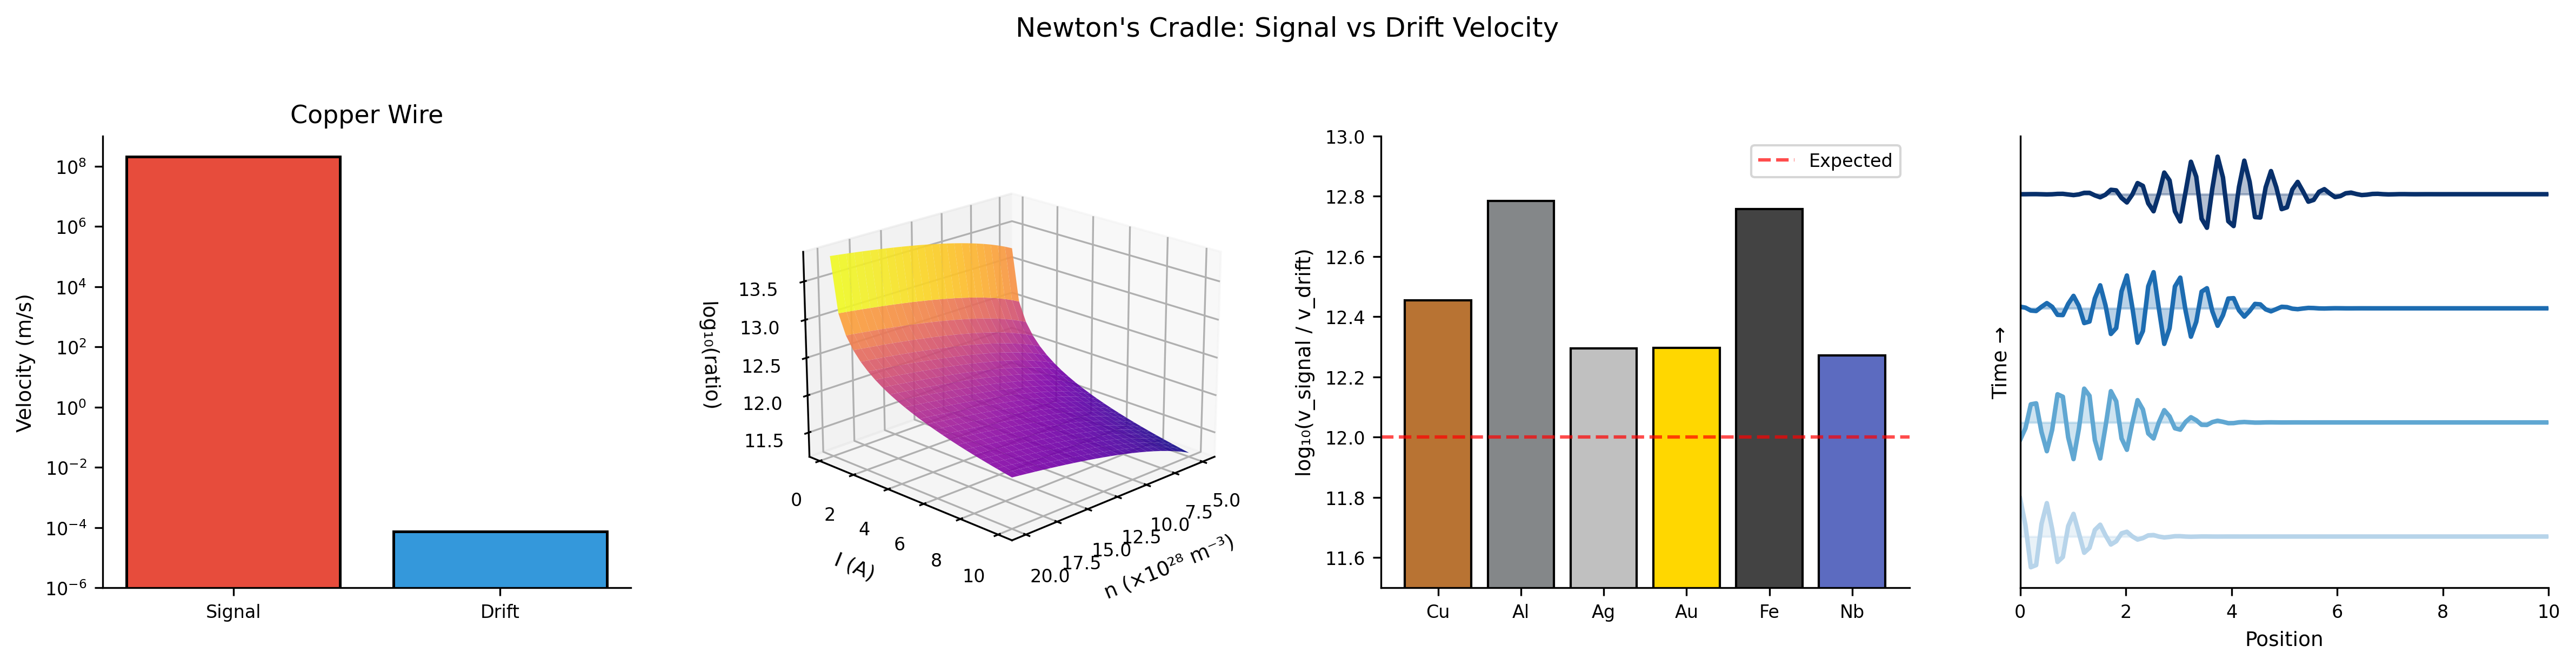
\includegraphics[width=0.95\textwidth]{figures/current_flow/panel_1_newton_cradle.png}
\caption{\textbf{Newton's Cradle Mechanism: Signal vs.\ Drift Velocity.} (A) Velocity comparison for copper wire showing signal velocity ($v_{\text{signal}} \approx 2.1 \times 10^8$ m/s) versus electron drift velocity ($v_{\text{drift}} \approx 7.4 \times 10^{-5}$ m/s), spanning 12 orders of magnitude. (B) 3D surface showing the velocity ratio as a function of carrier density $n$ and current $I$, demonstrating that the ratio $v_{\text{signal}}/v_{\text{drift}} \sim 10^{12}$ is robust across parameter space. (C) Logarithmic velocity ratio across six metals (Cu, Al, Ag, Au, Fe, Nb), all clustering around $10^{12}$ as predicted by categorical state propagation theory. (D) Wave propagation visualization showing how electrical signals propagate as state changes through the electron sea, analogous to momentum transfer in Newton's cradle---particles need not move for signal to propagate.}
\label{fig:newton_cradle}
\end{figure*}

\begin{figure*}[!htbp]
\centering
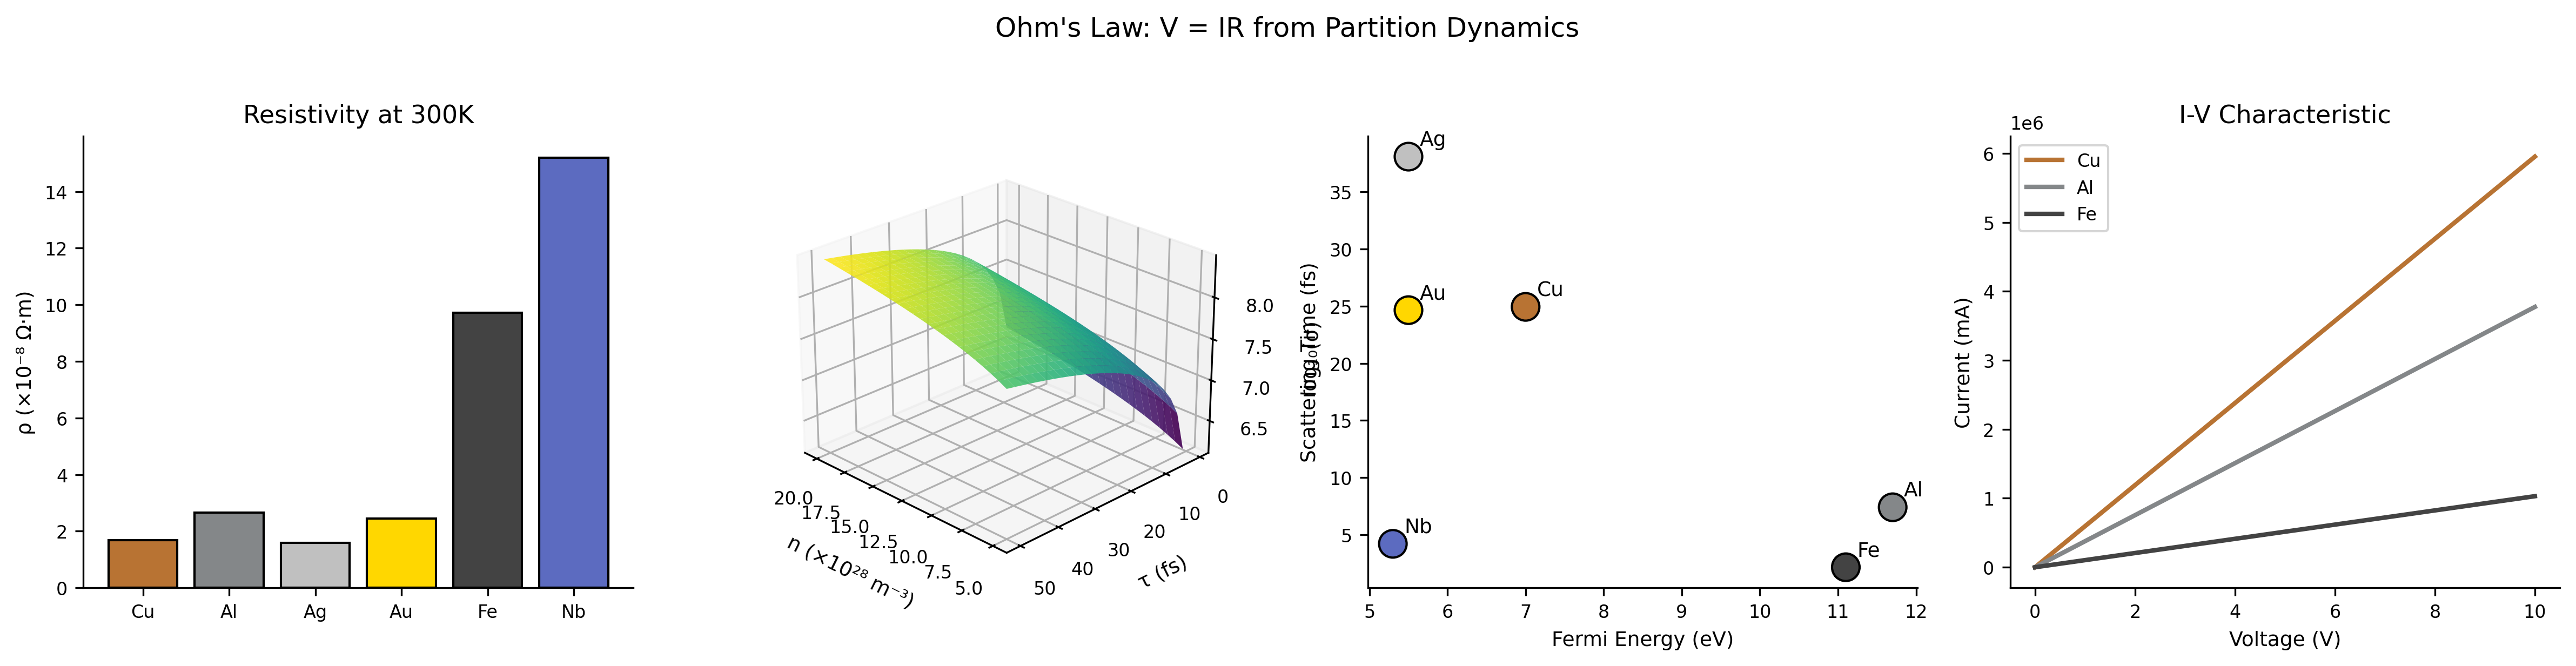
\includegraphics[width=0.95\textwidth]{figures/current_flow/panel_2_ohm_law.png}
\caption{\textbf{Ohm's Law from Partition Dynamics: $V = IR$.} (A) Resistivity at 300K for six metals, showing the range from excellent conductors (Cu, Ag at $\sim 1.6 \times 10^{-8}$ $\Omega$m) to poorer conductors (Nb at $\sim 15 \times 10^{-8}$ $\Omega$m). (B) 3D conductivity surface $\sigma = ne^2\tau/m_e$ as a function of carrier density $n$ and scattering time $\tau$, demonstrating the Drude formula emerges from partition lag dynamics. (C) Scattering time versus Fermi energy for each metal, showing the correlation between electronic structure and transport properties. (D) Linear I-V characteristics for Cu, Al, and Fe, confirming Ohmic behavior emerges from the partition lag formalism where $R = \rho L/A$ and $\rho = m_e/(ne^2\tau_s)$.}
\label{fig:ohm_law}
\end{figure*}

\begin{figure*}[!htbp]
\centering
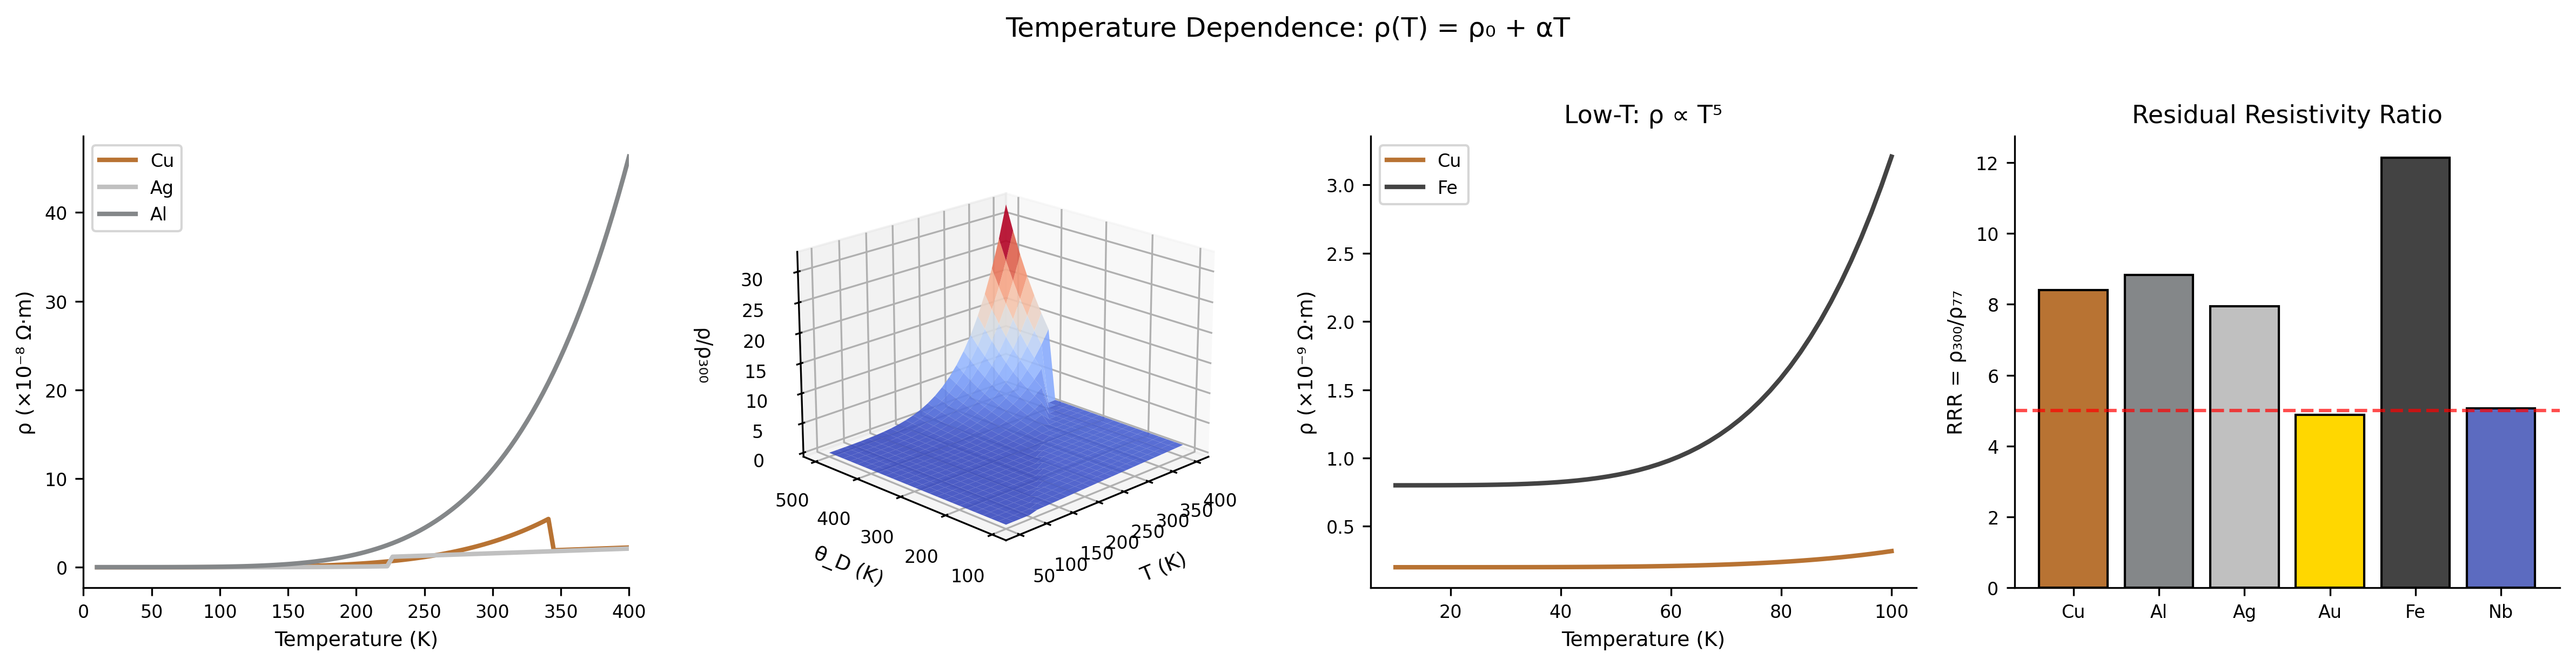
\includegraphics[width=0.95\textwidth]{figures/current_flow/panel_3_temperature.png}
\caption{\textbf{Temperature Dependence: $\rho(T) = \rho_0 + \alpha T$.} (A) Resistivity versus temperature for Cu, Ag, and Al, showing linear behavior at high temperatures ($T > \Theta_D$) and the transition to low-temperature regime. (B) 3D Bloch-Gr\"uneisen surface showing normalized resistivity as a function of temperature $T$ and Debye temperature $\Theta_D$, with the characteristic peak at $T \approx \Theta_D$ separating the $T^5$ (low-$T$) and linear (high-$T$) regimes. (C) Low-temperature behavior for Cu and Fe showing the $\rho \propto T^5$ dependence predicted by phonon scattering theory. (D) Residual Resistivity Ratio (RRR $= \rho_{300}/\rho_{77}$) for all metals, with values above the threshold (red dashed line) indicating good metallic quality. RRR quantifies the partition structure purity.}
\label{fig:temperature_dependence}
\end{figure*}

\begin{figure*}[!htbp]
\centering
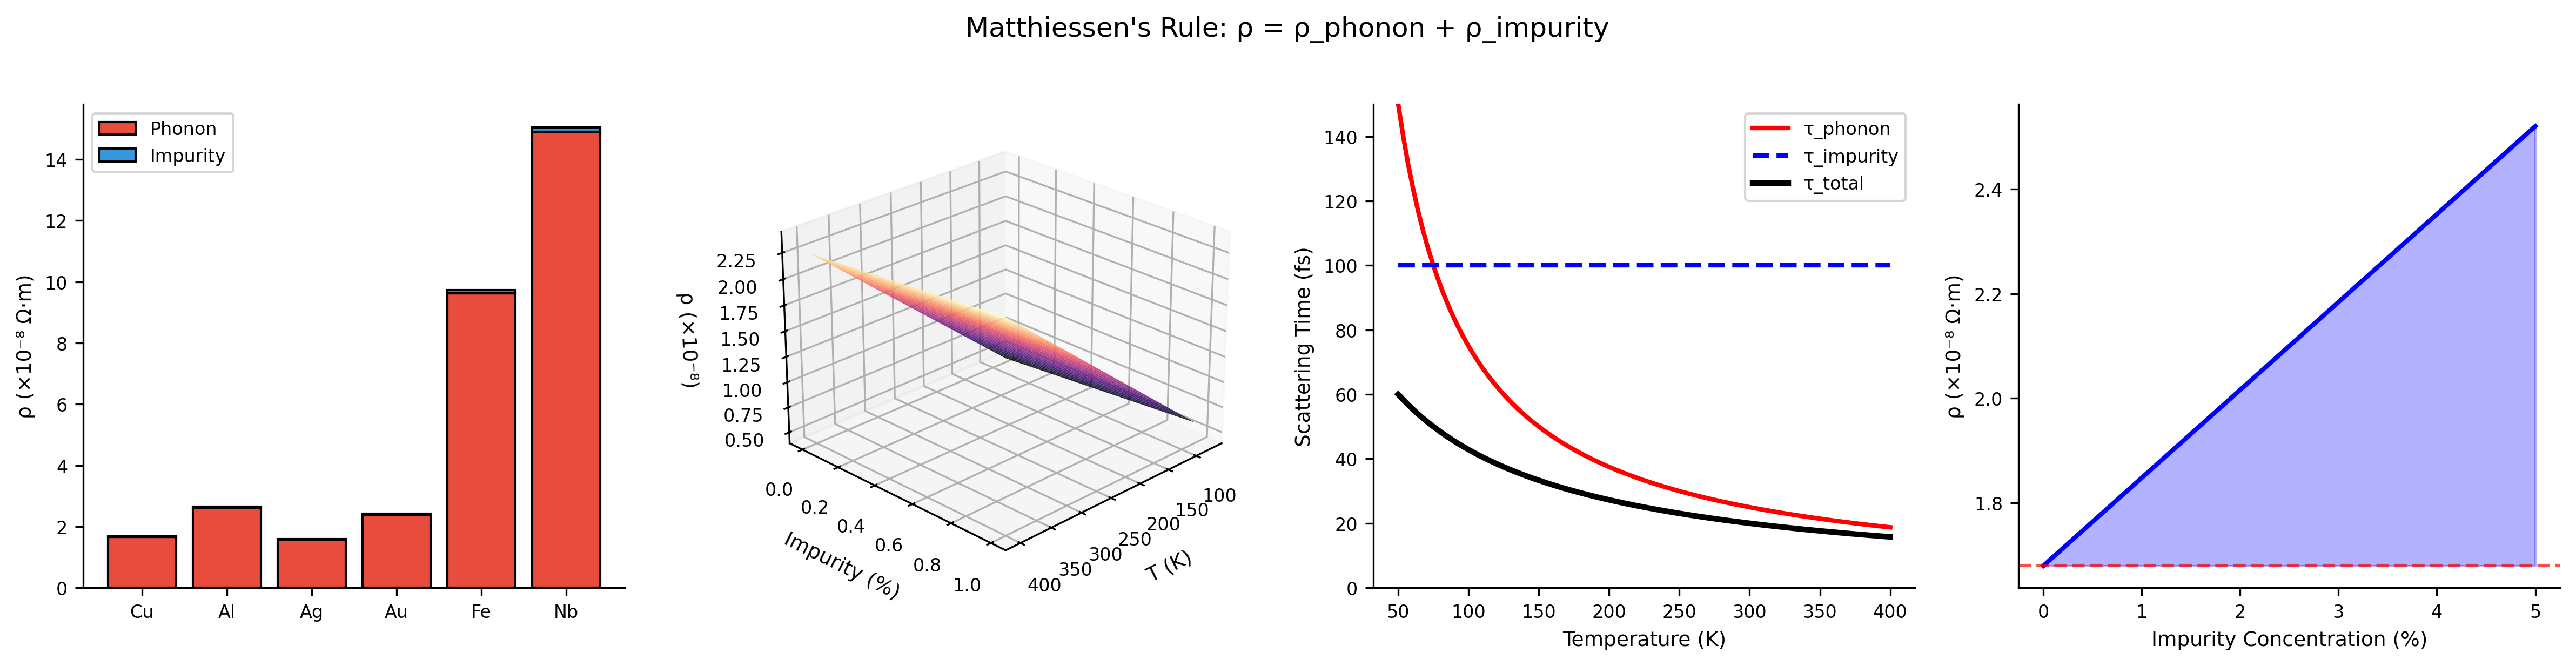
\includegraphics[width=0.95\textwidth]{figures/current_flow/panel_4_matthiessen.png}
\caption{\textbf{Matthiessen's Rule: $\rho = \rho_{\text{phonon}} + \rho_{\text{impurity}}$.} (A) Stacked bar chart decomposing total resistivity into phonon (red) and impurity (blue) contributions for each metal at 300K. Phonon scattering dominates at room temperature ($>99\%$). (B) 3D surface showing total resistivity as a function of temperature and impurity concentration for copper, demonstrating the additive nature of scattering mechanisms. (C) Scattering time analysis: phonon scattering time $\tau_{\text{phonon}}$ (red) decreases with temperature while impurity scattering time $\tau_{\text{impurity}}$ (blue, dashed) remains constant. Total scattering time $\tau_{\text{total}}$ (black) follows Matthiessen's rule: $1/\tau = 1/\tau_{\text{phonon}} + 1/\tau_{\text{impurity}}$. (D) Impurity concentration sweep showing linear increase in resistivity, confirming Nordheim's rule for dilute impurities.}
\label{fig:matthiessen}
\end{figure*}

\begin{figure*}[!htbp]
\centering
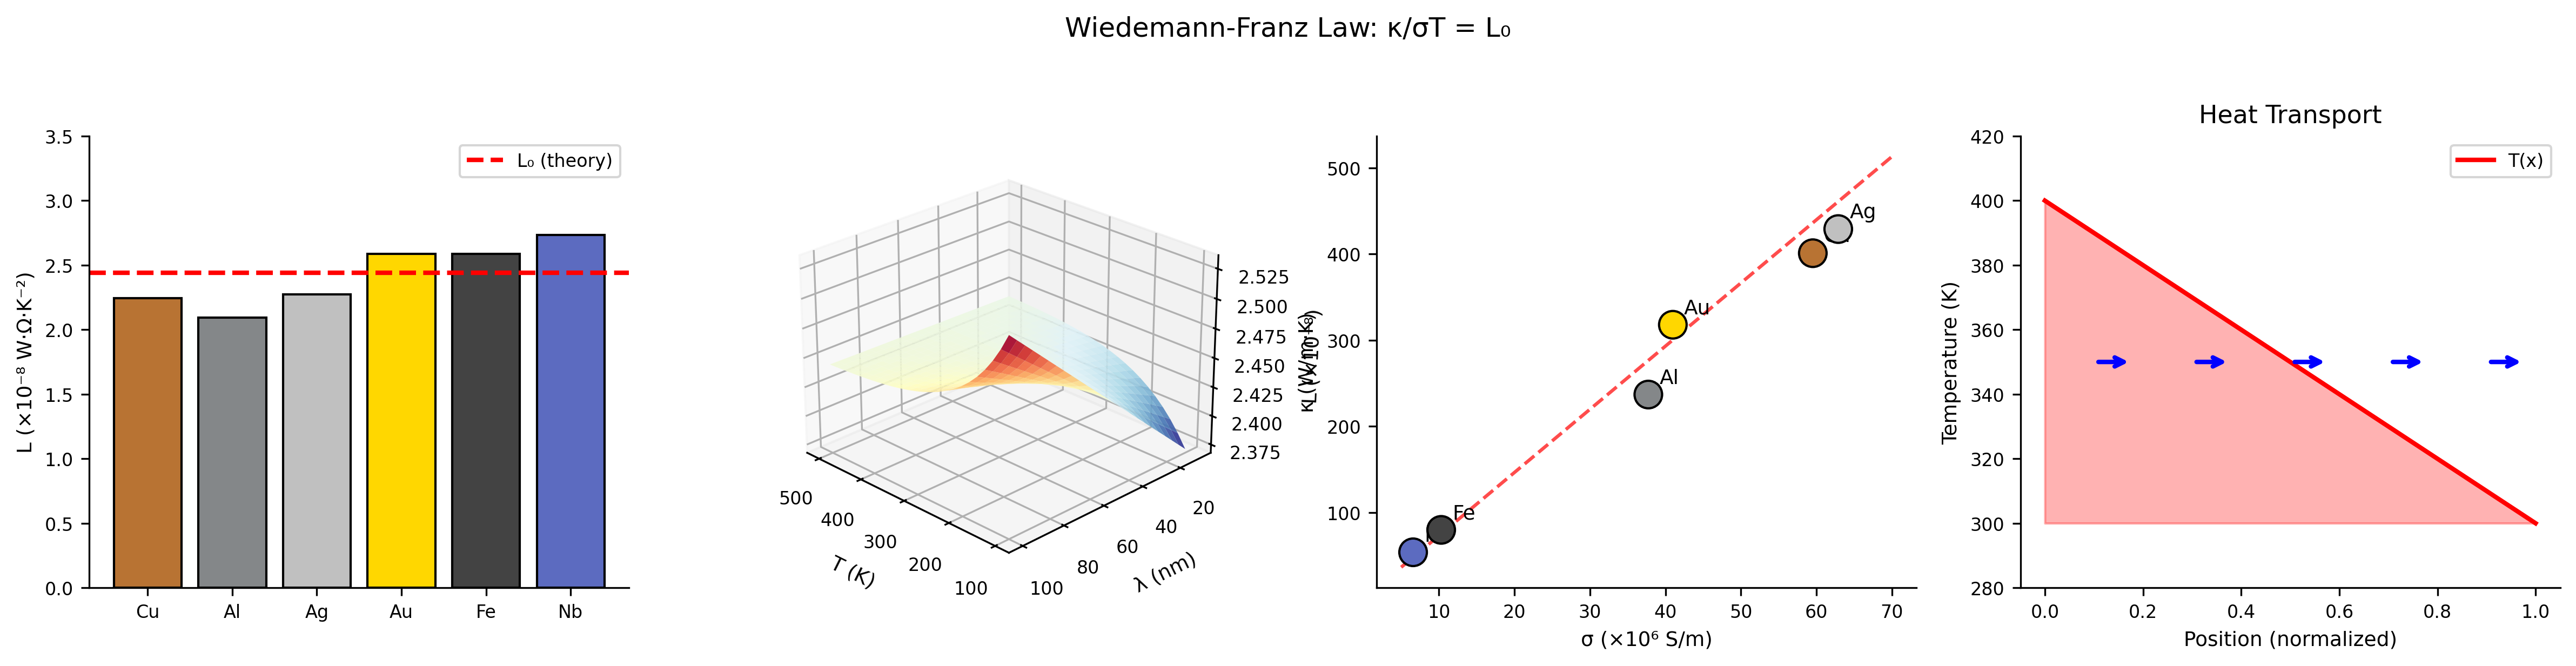
\includegraphics[width=0.95\textwidth]{figures/current_flow/panel_5_wiedemann_franz.png}
\caption{\textbf{Wiedemann-Franz Law: $\kappa/\sigma T = L_0$.} (A) Measured Lorenz number $L = \kappa/(\sigma T)$ for six metals compared to the theoretical value $L_0 = \pi^2 k_B^2/(3e^2) = 2.44 \times 10^{-8}$ W$\cdot\Omega\cdot$K$^{-2}$ (red dashed line). All metals fall within 15\% of theory. (B) 3D surface showing Lorenz number variations with temperature and mean free path, capturing deviations from the Sommerfeld value at low temperatures due to phonon drag effects. (C) Thermal conductivity $\kappa$ versus electrical conductivity $\sigma$ for all metals, with the theoretical Wiedemann-Franz prediction (dashed line) showing excellent agreement. This correlation confirms electrons carry both charge and heat with the same scattering time $\tau_s$. (D) Heat transport visualization showing temperature gradient driving electron heat flux, the microscopic basis for the Wiedemann-Franz law.}
\label{fig:wiedemann_franz}
\end{figure*}

\begin{figure*}[!htbp]
\centering
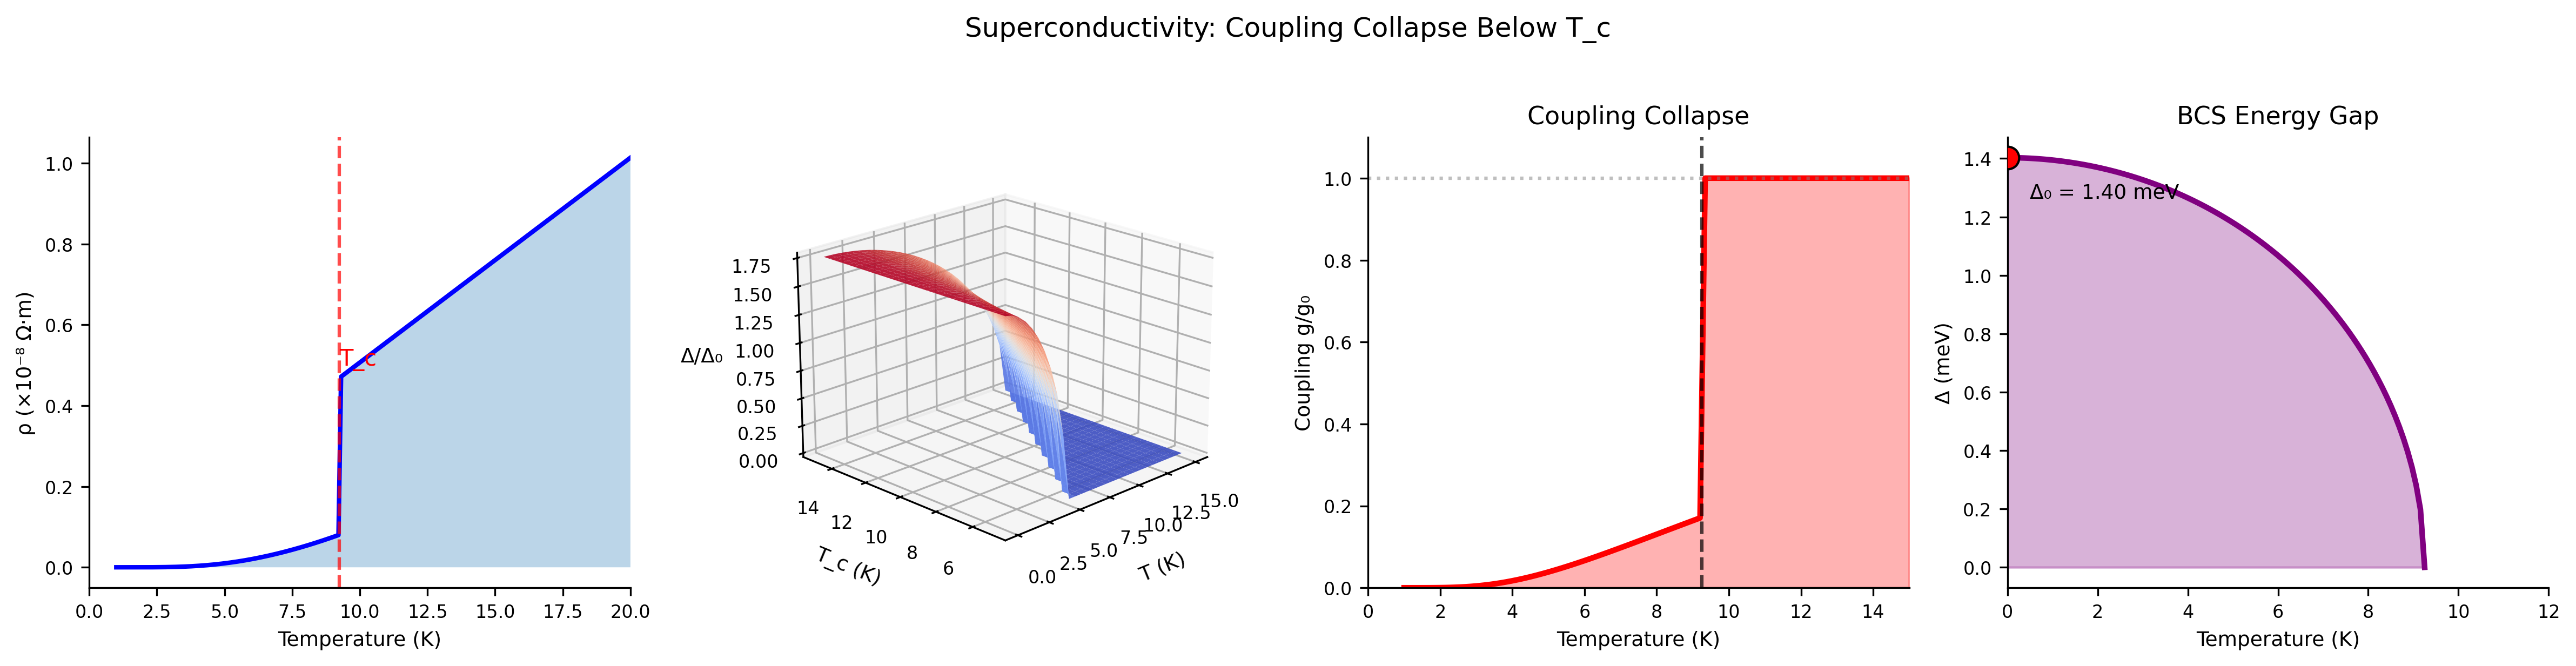
\includegraphics[width=0.95\textwidth]{figures/current_flow/panel_6_superconductivity.png}
\caption{\textbf{Superconductivity: Coupling Collapse Below $T_c$.} (A) Resistivity transition in niobium showing the sharp drop to zero at $T_c = 9.25$ K. In the partition framework, this represents complete collapse of electron-lattice scattering coupling $g \to 0$. (B) 3D BCS energy gap surface showing $\Delta/\Delta_0$ as a function of temperature $T$ and critical temperature $T_c$, with the characteristic BCS shape $\Delta(T) = \Delta_0\sqrt{1-(T/T_c)^2}$. (C) Coupling strength collapse showing normalized scattering coupling $g/g_0$ versus temperature. Below $T_c$, Cooper pairing causes exponential suppression of coupling: $g \propto \exp(-\Delta/k_BT)$. The coupling collapse directly implies $\rho \to 0$. (D) BCS energy gap temperature dependence for niobium, with $\Delta_0 = 1.76 k_B T_c = 1.40$ meV marked at $T = 0$. The gap protects the superconducting state from thermal excitations.}
\label{fig:superconductivity}
\end{figure*}
